\documentclass[11pt,a5paper]{article}

\usepackage[T1]{fontenc}
\usepackage[utf8]{inputenc}
\usepackage{lmodern, microtype}
\usepackage[estonian]{babel}

\usepackage{siunitx}
\sisetup{inter-unit-product=\ensuremath{{}\cdot{}}, per-mode=fraction, exponent-product=\cdot, output-decimal-marker={,}}

\usepackage{graphicx}
\usepackage{wrapfig}
\usepackage{subfig}
\usepackage{tikz}
\usetikzlibrary{patterns, patterns.meta}
\usetikzlibrary{arrows.meta}
\usepackage[european]{circuitikz}
\tikzset{component/.style={draw,thick,circle,fill=white,minimum size=0.75cm,inner sep=0pt}}
\usepackage{amsmath,amssymb}
\usepackage{amsfonts}
\usepackage[hidelinks]{hyperref}
\usepackage{csquotes}
\usepackage{caption}
\usepackage{enumitem}
\usepackage{wrapfig}
\topmargin=-3.0cm \textheight=19cm \textwidth=12.9cm
\oddsidemargin=-1.5cm  \evensidemargin=-1.5cm
\setlength{\parindent}{0pt} \setlength{\parskip}{6pt} \sloppy
\sloppy \relpenalty=10000 \binoppenalty=10000
\pagestyle{empty}

\newcommand{\numb}[1]{\vspace{5pt}\textbf{\large #1}}
\newcommand{\nimi}[1]{(\textsl{\small #1})}
\newcommand{\punktid}[1]{(\emph{#1~p.})}
\newcounter{ylesanne}
\newcommand{\yl}[1]{\addtocounter{ylesanne}{1}\numb{\theylesanne.} \nimi{#1} \newblock{}}
\newcommand{\autor}[1]{}% Kasuta võistluse ajal
%\newcommand{\autor}[1]{\emph{ Autor: #1}}% Kasuta kui vaja autorit

\begin{document}
\begin{center}
  \textbf{\Large Eesti koolinoorte 35.\ füüsika lahtine võistlus} \par
  \emph{30.\ november 2024. a.\\Vanema rühma ülesanded (11.--12.\ klass)}
\end{center}

\resizebox{\textwidth}{!}{
  \emph{%
    \begin{tabular}{@{}l@{}}
      \textbf{Palun kirjutada iga ülesande lahendus eraldi lehele.}\\
      Lahendamisaeg on 5 tundi. \\
      Iga osavõtja võib lahendada kõiki pakutud ülesandeid. \\
      Arvesse lähevad 6 suurima punktide arvu saanud lahendust. \\
      Kasutada võib kirjutus- ja joonestusvahendeid ning kalkulaatorit. Muud abivahendid on keelatud.\\
    \end{tabular}
  }
} \par



\yl{VABASUKELDUMINE}
Vabasukeldumise sügavusrekordit püüdes peab sukelduja alguses sügavuse kasvamiseks palju vaeva nägema, kuna vee üleslükejõud surub vastu. Mingi hetk hakkab sukelduja vabalangema, sest sukelduja ruumala väheneb kokkusurutud kopsude arvelt. Leia kui sügavalt alates hakkab sukelduja vabalangema. Sukeldaja mass on $m_0 = \SI{75}{\kg}$, õhku täistõmmatud kopsude ruumala on $V_{k} = \SI{12}{\l}$ ja sellel hetkel on sukelduja koguruumala $V_0 = \SI{84}{\l}$. Eelda, et sukelduja temperatuur ei muutu sukelduse ajal ja rinnakorvi elastusjõud ei mõjuta kopsuruumala. Õhurõhk on $P_0 = \SI{101300}{\Pa}$, raskuskiirendus on $g = \SI{9.8}{\m\per\s\squared}$ ja vee tihedus on $\rho = \SI{1000}{\kg\per\m\cubed}$
\punktid{6} \autor{Jarl Patrick Paide}





\yl{KAKS KERA}
Kaks sama tiheduse ja ühtlase massijaotusega kera peaaegu puutuvad üksteist (keskpunktide vaheline kaugus on kaks raadiust), aga hõõrdumist ei toimu. Kerad tiirlevad ümber üksteise gravitatsioonijõu tõttu nurkkiirusega $\omega$. Leia kerade tihedus.
\punktid{6} \autor{Jarl Patrick Paide}



\yl{VALGUSKAABEL}
Silindriline sirge valguskaabel koosneb südamikust ja kattekihist ning selle ots on tasane ja kaabliga risti. Kui valgustada kaabli otsa välise valgusallikaga, siseneb osa välisest valgusest südamikku ja levib praktiliselt kadudeta pikki vahemaid. Seda, kui vastuvõtlik on valguskaabel välisele valgusele, iseloomustab numbriline apertuur (NA), mis on defineeritud kui $\text{NA} = \sin \theta_0$, kus $\theta_0$ on suurim välise valguskiire nurk (kaabli sümmeetriatelje suhtes), mis valguskaablisse sisenedes levib selle südamikus kadudeta. Leia valguskaabli numbriline apertuur NA, kui südamiku murdumisnäitaja on $n_1$, kattekihi murdumisnäitaja on $n_2$ ja kaabel asub välises keskkonnas murdumisnäitajaga $n_0$.
\punktid{8} \autor{Richard Luhtaru}
\begin{figure}[h]
    \centering
    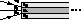
\includegraphics[width=.7\linewidth]{valguskaabel_joonis.pdf}
\end{figure}



\yl{RONGIÜHENDUS}
Raudteelõigul sõidavad rongid pikkusega $l=\SI{900}{\m}$. Millise kiirusega peaksid rongid sõitma, et raudteelõigu läbilaskmisvõime oleks maksimaalne (s.t. päevas läbib raudteelõiku nii palju ronge kui võimalik) ja ohutu vahekaugus rongide vahel oleks tagatud? Lihtsustatult eeldada, et kahe sõitva rongi vaheline ohutu kaugus on kaks korda suurem kui vahemaa, mis kulub tagumisel rongil seisma jäämiseks. Rongid pidurdavad kiirendusega $a=\SI{1}{\m\per\s\squared}$. Eeldada, et rongid sõidavad kogu raudteelõigu pikkuses ühtlase kiirusega üksteise järel ühes suunas. \\
\textit{Vihje: Kasuks võib tulla võrratus $x+y \geq 2\sqrt{xy}$ kui $x, y \geq 0$.}
\punktid{10} \autor{Jonatan Kalmus}



\yl{VÄRSKE ÕHK}
Anu hoiab õhutusakna osaliselt lahti, parasjagu nii palju, et süsihappegaasi sisaldus toas ei oleks suurem, kui 1000 ppm. Lühend ppm tähendab ``osakest miljoni kohta'', st antud juhul ei tohi iga miljoni õhumolekuli kohta olla õhus rohkem, kui 1000 süsihappegaasi molekuli. Õueõhus on süsihappegaasi sisaldus 420 ppm ja temperatuur  $t_0=\SI{-10}{\celsius}$ ja õhurõhk $p=\SI{1e5}{\pascal}$. Toas on kolm inimest, kellest igaüks toodab $v=\SI{17}{\litre\per\hour}$  süsihappegaasi. Millise võimsusega on vaja tuba kütta, et hoida toatemperatuur $t_1=\SI{20}{\celsius}$ juures? Soojuskaudega läbi aknaklaaside, seinte jms mitte arvestada.
\punktid{10} \autor{Jaan Kalda}



\begin{wrapfigure}{r}{0.4\textwidth}
\vspace{-0.8cm}
  \begin{center}
    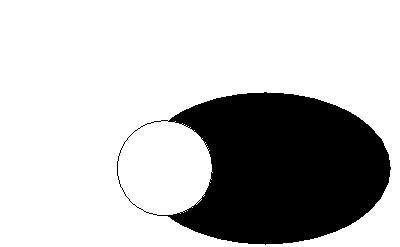
\includegraphics[width=1\linewidth]{vari.pdf}
  \end{center}
  \vspace{-0.9cm}
\end{wrapfigure}

\yl{VARI}
Joonisel (suurem koopia lisalehel) on näidatud ülaltvaates horisontaalsel laual lebav kera ja selle vari, mille heidab lauale punktvalgusallikas. Mitme kera raadiuse kaugusel kera keskpunktist asub see punktvalgusallikas? Võite teha joonisel lisakonstruktsioone ja mõõtmisi.
\punktid{10} \autor{Jaan Kalda}



\yl{ÄIKESETORM}
Helena mõõtis äikesetormi ajal Maa magnetvälja väga täpse elektroonilise magnetomeetriga. Ta hakkas muretsema äikesetormi mõjudest mõõtmistele ja otsustas seda uurida. Äikese sähvatusest kuni heli saabumiseni läks aega $t = \SI{10}{\s}$. Ta uuris välja, et tavalise äikselöögi voolutugevus on $I = \SI{30000}{\ampere}$, õhu magneetiline läbitavus on $\mu = \SI{1.26e-6}{\tesla\metre\per\ampere}$ ja heli kiirus õhus on $v_{õ} = \SI{340}{\m\per\s}$. Leia mitu kraadi maksimaalselt muutub mõõteriista poolt mõõdetud põhja suund löögi hetkel. Tavakeskkonnas magneomeeter mõõdab Maa magnetvälja tugevuseks $B = \SI{50}{\micro \tesla}$ ning magnetväli moodustab vertikaalse sihiga nurga $\alpha = 17^{\circ}$. \\
\textit{Vihje:} Sirge juhe voolutugevusega $I$ tekitab endast kaugusele $r$ magnetvälja tugevusega $B = \frac{\mu I}{2\pi r}$. Tekkinud magnetvälja suund on risti juhtmega ja tangensiaalne vastavalt kruvireeglile.
\punktid{10} \autor{Jarl Patrick Paide}




\yl{KÄRU}
Kilplased ehitasid käru, mille esimeste ja tagumiste rataste vahel on jõuülekanne: kui esimesi rattaid pöörata päripäeva 8 pööret, teevad tagumised rattad päripäeva 9 pööret. Millise maksimaalse kaldenurgaga teel püsib see käru ilma alla libisemata paigal, kui hõõrdetegur rataste ja tee vahel on  $\mu$ ning esimestele ja tagumistele ratastele mõjub tee poolt ühesugune  toereaktsioon?
\punktid{12} \autor{Jaan Kalda}





\yl{KONDENSAATORID}
Kaks ruudukujulise plaadiga õhkkondensaatorit on ühendatud jadamisi ning neile on rakendatud alalispinge $U$. Kondensaatorite plaatide küljepikkused on vastavalt $b$ ja $2b$ ning plaatidevaheline kaugus on $d$, kusjuures $d \ll b$. Kahe kondensaatori vaheline kaugus on $b$. Kondensaatoreid läbib plaadiga paralleelse algkiirusega $v_0$ osake laenguga $q$ ja massiga $m$. Milline on osakese nihe kondensaatori telje sihis, kui ta väljub teise kondensaatori piirkonnast? Eeldage, et osake läbib mõlemat kondensaatorit nende plaate puutumata. Raskuskiirenduse ja kondensaatori ääreefektidega arvestama ei pea. \\
\textit{Vihje:} Kondensaatori mahtuvus on $C=\frac{\varepsilon\varepsilon_0S}{d}$.
\punktid{12} \autor{Uku Andreas Reigo}

\begin{center}
\begin{circuitikz}[european]
\ctikzset{bipoles/cuteswitch/thickness=0.5}
\draw
(0,2) to[short] (0,6)
to[short] (2,6)
to[C] (2,4)
to[short, l^= $b$] (3,4)
to[short](4,4)
to[short] (4,4.85);
\draw
(4,5.15) to [short] (4,6)
to[short, l_ = $2b$] (6,6);

\draw
(0,2) to [battery1, l^ = $U$] (6,2)
to [short] (6,6);

\draw[line width = 1]
(3.25,5.15) to [short] (4.75,5.15);
\draw[line width = 1]
(3.25,4.85) to [short] (4.75,4.85);

\draw[-latex, dashed]
(0.25,5) node[below right] {$m,q$} to [short, l^=$v_0$]  (1.25,5) ;

\end{circuitikz}
\end{center}

\yl{PÄRITUUL}
Jalgrattur sõidab mööda teed.  Samal ajal puhub pooleldi selja tagant tuul, mille kiirus on täpselt võrdne jalgratturi kiirusega; tuule suund moodustab tee sihiga nurga $\alpha<90^\circ$. Milliste nurga $\alpha$ väärtuste puhul tuul takistab sõitmist (st rattur saaks tuulevaikse ilmaga sama kiiresti sõita kulutades õhutakistuse ületamiseks väiksemat võimsust)? Lugeda, et õhu takistusjõud on võrdeline ratturi kiiruse ruuduga õhu suhtes.
\punktid{12} \autor{Jaan Kalda}

\end{document}

